\chapter{Experimentación}\label{cap:experimentacion}

\section{Experimentos preliminares}

En esta primera fase de experimentacion se realizarán pruebas para determinar los parámetros óptimos de ejecución y estudiar el rendimiento de la aplicación en distintos entornos y plataformas.

\subsection{Determinación del número óptimo de subpoblaciones y hebras}

Como se ha comentado en la sección \ref{subsubsec:determinacion_subpoblaciones}, se realizarán ejecuciones exploratorias con distintas configuraciones de subpoblaciones y hebras, para definir el parámetro de \texttt{NSubpopulations} a usar en los tests posteriores.

En la figura \ref{fig:exploratory_subpopulations} se muestran las gráficas de estas ejecuciones exploratorias. Se observa que para cualquier número de subpoblaciones, el comportamiento es similar. En la tabla \ref{tab:exploratory_subpopulations_times} se presentan los tiempos de ejecución en segundos para cada combinación de hebras y subpoblaciones, mostrando cómo el incremento en el número de subpoblaciones aumenta significativamente el tiempo de ejecución, especialmente cuando se utilizan pocas hebras.

\begin{figure}[ht]
    \centering
    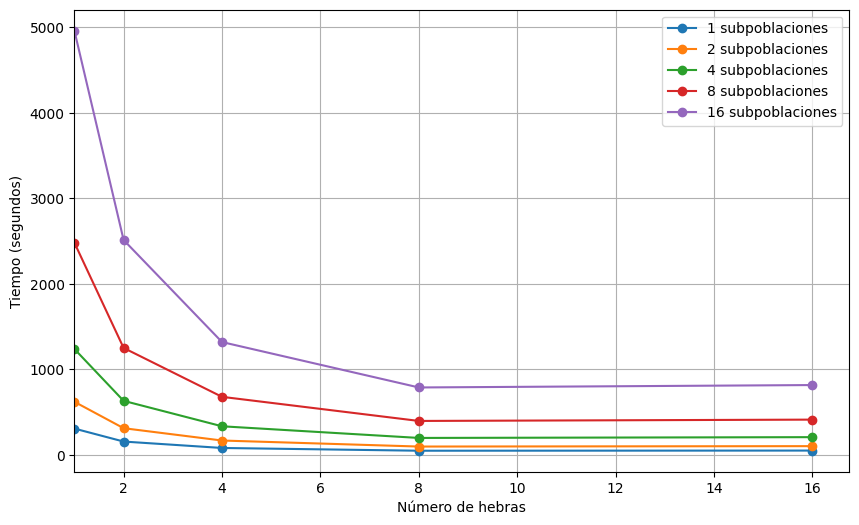
\includegraphics[width=0.8\textwidth]{imagenes/cap5/exploratory_subpopulations.png}
    \caption{Gráficas de ejecución de las pruebas variando el número de subpoblaciones y hebras.}
    \label{fig:exploratory_subpopulations}
\end{figure}

\begin{table}[ht]
    \centering
    \begin{tabular}{|c|ccccc|}
        \hline
        \multirow{2}{*}{\textbf{Hebras}} & \multicolumn{5}{c|}{\textbf{Subpoblaciones}}                                                      \\ \cline{2-6}
                                         & \textbf{1}                                   & \textbf{2} & \textbf{4} & \textbf{8} & \textbf{16} \\ \hline
        1                                & 309.43                                       & 622.63     & 1239.73    & 2481.89    & 4960.00     \\ \hline
        2                                & 157.79                                       & 313.86     & 633.66     & 1252.12    & 2513.72     \\ \hline
        4                                & 82.73                                        & 169.76     & 336.25     & 680.46     & 1320.66     \\ \hline
        8                                & 50.58                                        & 99.37      & 200.01     & 398.66     & 790.04      \\ \hline
        16                               & 52.32                                        & 104.06     & 209.17     & 414.11     & 818.17      \\ \hline
    \end{tabular}
    \caption{Tiempos de ejecución en segundos de las pruebas variando el número de subpoblaciones y hebras.}
    \label{tab:exploratory_subpopulations_times}
\end{table}

En la tabla \ref{tab:exploratory_populations_delta} se presentan los porcentajes de reducción del tiempo de ejecución respecto a la configuración base. En cada columna, la ejecución con una sola hebra y una sola subpoblación se toma como referencia (0\% de reducción). Estos resultados permiten cuantificar de manera objetiva el beneficio relativo derivado del incremento del paralelismo y de la subdivisión de la población, proporcionando una base empírica para identificar configuraciones óptimas de ejecución.

\begin{table}[ht]
    \centering
    \begin{tabular}{|c|ccccc|}
        \hline
        \multirow{2}{*}{\textbf{Hebras}} & \multicolumn{5}{c|}{\textbf{Subpoblaciones}}                                                      \\ \cline{2-6}
                                         & \textbf{1}                                   & \textbf{2} & \textbf{4} & \textbf{8} & \textbf{16} \\ \hline
        1                                & 0.00                                         & 0.00       & 0.00       & 0.00       & 0.00        \\ \hline
        2                                & -49.01                                       & -49.59     & -48.89     & -49.55     & -49.32      \\ \hline
        4                                & -73.26                                       & -72.74     & -72.88     & -72.58     & -73.37      \\ \hline
        8                                & -83.65                                       & -84.04     & -83.87     & -83.94     & -84.07      \\ \hline
        16                               & -83.09                                       & -83.29     & -83.13     & -83.31     & -83.50      \\ \hline
    \end{tabular}
    \caption{Porcentaje de reducción del tiempo de ejecución respecto a la configuración base para distintas combinaciones de hebras y subpoblaciones}
    \label{tab:exploratory_populations_delta}
\end{table}

Del análisis de esta tabla pueden extraerse varias conclusiones de interés para la definición de los parámetros en los experimentos posteriores. En primer lugar, se observa que, para un número fijo de hebras, la variación en el porcentaje de reducción del tiempo es prácticamente inexistente al modificar el número de subpoblaciones, lo que indica que el comportamiento es proporcional con independencia de este parámetro. En segundo lugar, el mayor beneficio en términos de reducción del tiempo de ejecución se obtiene al incrementar el número de hebras de 1 a 8, alcanzando valores en torno al 83--84\%. Sin embargo, al pasar de 8 a 16 hebras, los tiempos de ejecución se incrementan en todos los casos, lo que revela que se ha sobrepasado el punto de paralelismo óptimo para la arquitectura hardware utilizada. Este resultado sugiere que, en el entorno experimental considerado, el uso de más de 8 hebras no proporciona mejoras de rendimiento adicionales e, incluso, puede resultar contraproducente debido a la sobrecarga y la contención de recursos.

No obstante, se ha decidido mantener configuraciones con 16 hebras en los experimentos posteriores con el fin de analizar el comportamiento bajo condiciones de sobrecarga, dado que el objetivo del estudio trasciende la mera optimización de un caso específico y busca evaluar la escalabilidad y el rendimiento en un rango amplio de escenarios. En cuanto al número de subpoblaciones, se constata que con 16 subpoblaciones los tiempos de ejecución pueden alcanzar hasta 1 hora y 20 minutos en configuraciones con una única hebra, lo que resulta excesivo para los objetivos de este trabajo. Por el contrario, con 8 subpoblaciones se obtienen tiempos de ejecución más razonables, se alcanza un equilibrio adecuado entre eficiencia y aprovechamiento de recursos, y se garantiza una buena escalabilidad.

En consecuencia, se justifica la decisión metodológica de fijar el número de subpoblaciones en 8 para los experimentos posteriores, al representar un compromiso óptimo entre eficiencia, utilización de recursos y escalabilidad en el entorno analizado.

\subsection{Estudio del rendimiento al requerir más hebras de las disponibles}

En esta sección se presentan los resultados de las ejecuciones exploratorias realizadas para analizar el rendimiento de la aplicación al variar el número de nodos y hebras, incluyendo configuraciones que superan el límite físico de hebras de la CPU (16 hebras). El objetivo es comprender cómo afecta esta variación al tiempo de ejecución y al uso efectivo de la CPU, proporcionando una base para la selección de parámetros en estudios posteriores.

En la figura \ref{fig:exploratory_threads_limit_time} se muestra la evolución del tiempo de ejecución en función del número de hebras asignadas por nodo, para configuraciones que van desde 1 hasta 16 nodos, pero limitando el número máximo de hebras a 16.

\begin{figure}[ht]
    \centering
    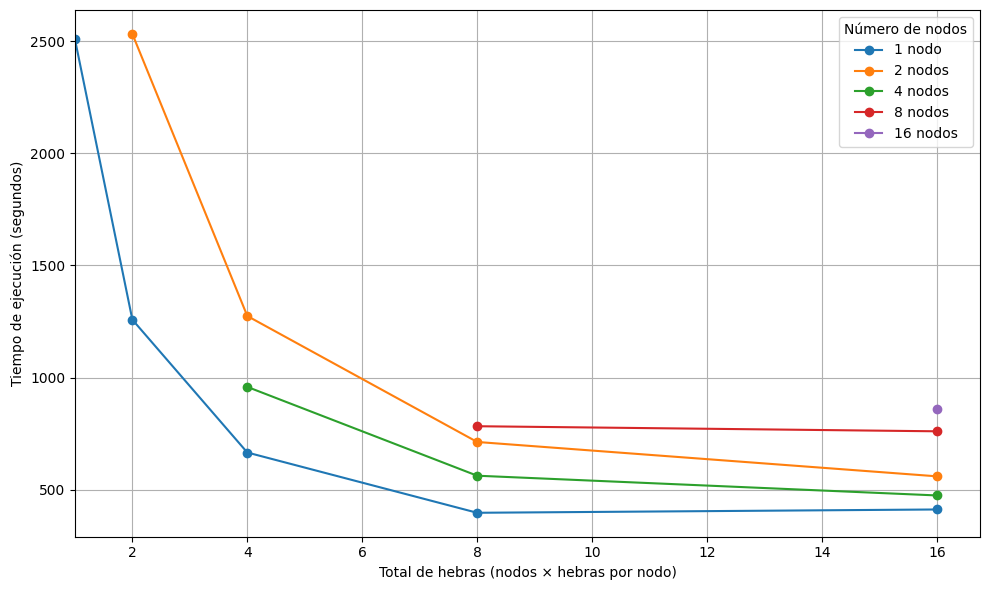
\includegraphics[width=0.8\textwidth]{imagenes/cap5/exploratory_threads_limit_time.png}
    \caption{Gráfica de tiempo de ejecución en función del número de hebras por nodo, con límite de 16 hebras.}
    \label{fig:exploratory_threads_limit_time}
\end{figure}

La figura \ref{fig:exploratory_threads_limit_cpu} muestra el porcentaje de uso total de CPU (donde 100\% equivale al uso completo de una hebra) para las distintas configuraciones de hebras por nodo analizadas.

\begin{figure}[ht]
    \centering
    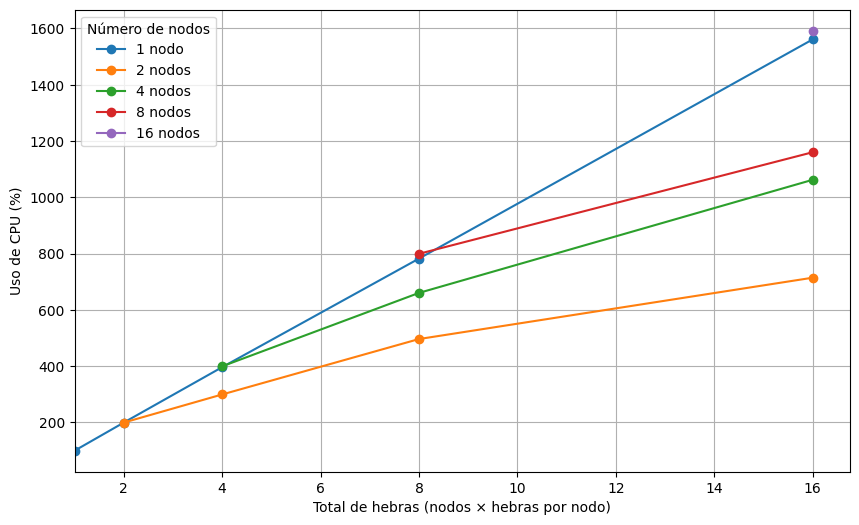
\includegraphics[width=0.8\textwidth]{imagenes/cap5/exploratory_threads_limit_cpu.png}
    \caption{Gráfica de uso de CPU en función del número de hebras por nodo, con límite de 16 hebras.}
    \label{fig:exploratory_threads_limit_cpu}
\end{figure}

Por otro lado, en la figura \ref{fig:exploratory_threads_no-limit_time} se presentan los resultados de las ejecuciones exploratorias sin límite en el número de hebras, permitiendo así evaluar el comportamiento del sistema al requerir más hebras de las disponibles.

\begin{figure}[ht]
    \centering
    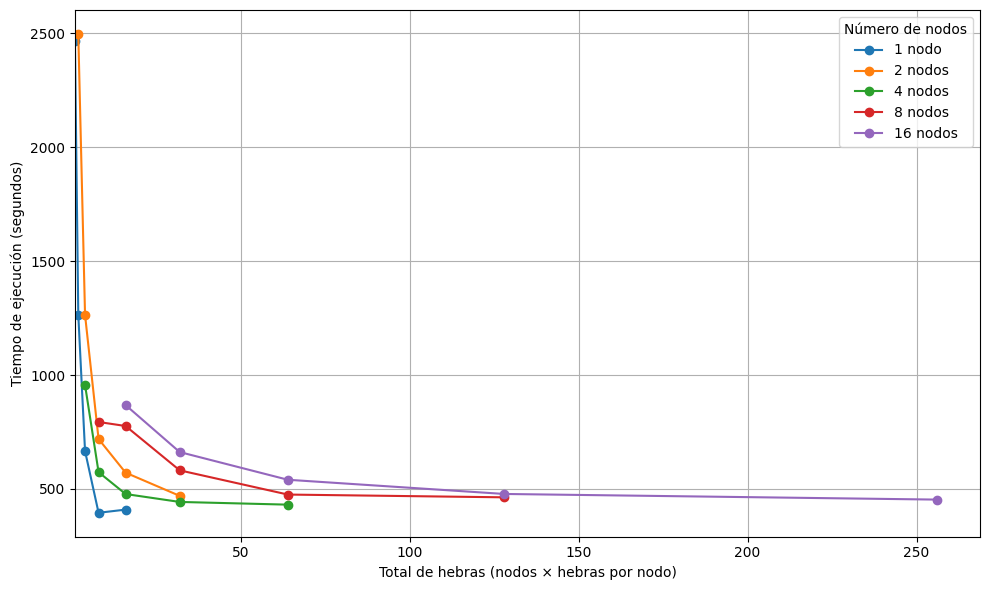
\includegraphics[width=0.8\textwidth]{imagenes/cap5/exploratory_threads_no-limit_time.png}
    \caption{Gráfica de tiempo de ejecución en función del número de hebras por nodo, sin límite en el número de hebras.}
    \label{fig:exploratory_threads_no-limit_time}
\end{figure}

La figura \ref{fig:exploratory_threads_no-limit_cpu} muestra el porcentaje de uso total de CPU para las distintas configuraciones de hebras por nodo sin límite, permitiendo observar cómo varía el aprovechamiento de los recursos en función del número total de hebras asignadas.

\begin{figure}[ht]
    \centering
    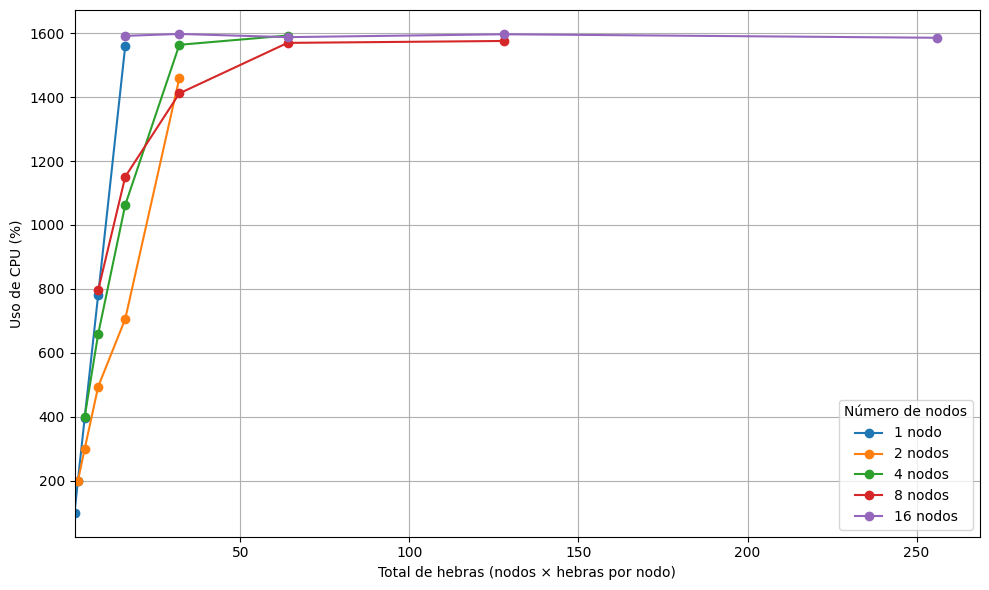
\includegraphics[width=0.8\textwidth]{imagenes/cap5/exploratory_threads_no-limit_cpu.png}
    \caption{Gráfica de uso de CPU en función del número de hebras por nodo, sin límite en el número de hebras.}
    \label{fig:exploratory_threads_no-limit_cpu}
\end{figure}

Las conclusiones que se pueden extraer de estas gráficas se pueden ver de manera más clara en la tabla \ref{tab:summary_nodes_threads_cpu}, donde se resumen los tiempos de ejecución y el uso de CPU para todas las combinaciones de nodos y hebras analizadas, tanto con límite como sin límite en el número de hebras.

\begin{table}[ht]
    \centering
    \small
    \setlength{\tabcolsep}{4pt}
    \renewcommand{\arraystretch}{1.1}
    \begin{tabular}{|c|c|c|c|c|}
        \hline
        \textbf{Nodos} & \textbf{Hebras}   & \textbf{Hebras}  & \textbf{Tiempo} & \textbf{Uso de}   \\
                       & \textbf{por nodo} & \textbf{totales} & \textbf{(s)}    & \textbf{CPU (\%)} \\
        \hline
        1              & 8                 & 8                & 395.63          & 782               \\
        1              & 16                & 16               & 409.51          & 1561              \\
        4              & 16                & 64               & 431.30          & 1593              \\
        4              & 8                 & 32               & 443.23          & 1564              \\
        16             & 16                & 256              & 453.48          & 1586              \\
        8              & 16                & 128              & 463.45          & 1576              \\
        2              & 16                & 32               & 469.88          & 1460              \\
        8              & 8                 & 64               & 475.59          & 1570              \\
        4              & 4                 & 16               & 477.90          & 1063              \\
        16             & 8                 & 128              & 478.23          & 1597              \\
        16             & 4                 & 64               & 540.54          & 1588              \\
        2              & 8                 & 16               & 571.65          & 706               \\
        4              & 2                 & 8                & 573.94          & 659               \\
        8              & 4                 & 32               & 581.91          & 1412              \\
        16             & 2                 & 32               & 662.10          & 1598              \\
        1              & 4                 & 4                & 666.51          & 396               \\
        2              & 4                 & 8                & 719.43          & 494               \\
        8              & 2                 & 16               & 776.44          & 1151              \\
        8              & 1                 & 8                & 794.09          & 796               \\
        16             & 1                 & 16               & 868.28          & 1592              \\
        4              & 1                 & 4                & 956.38          & 399               \\
        2              & 2                 & 4                & 1263.74         & 299               \\
        1              & 2                 & 2                & 1264.94         & 199               \\
        1              & 1                 & 1                & 2467.76         & 99                \\
        2              & 1                 & 2                & 2497.06         & 199               \\
        \hline
    \end{tabular}
    \caption{Resumen de configuraciones de nodos, hebras y uso de CPU}
    \label{tab:summary_nodes_threads_cpu}
\end{table}

Los resultados muestran que el mejor rendimiento se alcanza empleando un menor número de nodos con un mayor número de hebras por nodo, siendo la configuración óptima la de un único nodo y ocho hebras. Aunque el límite físico de hebras de la CPU es de 16, se observa que, entre los diez mejores resultados, solo tres respetan este límite. En los demás casos, incrementar el número de hebras más allá de la capacidad física sigue proporcionando mejoras en el rendimiento, un comportamiento que, aunque inicialmente contraintuitivo, puede explicarse analizando el uso efectivo de la CPU.

El porcentaje de utilización de la CPU refleja el grado de aprovechamiento de las hebras disponibles: por ejemplo, con una hebra se alcanza un uso máximo de 100\%, con dos hebras el 200\%, y así sucesivamente hasta un máximo teórico de 1600\% (16 hebras $\times$ 100\%). En configuraciones de un único nodo, aumentar el número de hebras se traduce en un incremento proporcional del uso de CPU, lo que explica las mejoras de rendimiento observadas.

En contraste, cuando el número total de hebras se distribuye entre varios nodos, incluso si no se supera el límite físico de la CPU, el rendimiento no mejora de la misma manera. Esto se debe a la sobrecarga inherente a la gestión de múltiples nodos, que puede contrarrestar los beneficios de disponer de más hebras, haciendo que el uso efectivo de la CPU no alcance los valores esperados y resultando en un rendimiento inferior respecto a configuraciones mononodo equivalentes. Por tanto, para configuraciones multinodo es necesario incrementar el número de hebras más allá de la capacidad física de cada CPU para acercarse al uso máximo teórico, lo que explica por qué los mejores resultados se obtienen bajo estas condiciones.

\subsection{Estudio del rendimiento al utilizar la misma GPU en distintos nodos}

En esta sección se presentan los resultados de las ejecuciones exploratorias realizadas para analizar el rendimiento de la aplicación al variar el número de nodos y hebras, considerando dos enfoques distintos respecto al uso de la GPU: uno en el que se limita su uso a un único nodo y otro en el que se permite su uso en todos los nodos. El objetivo es comprender cómo afecta esta variación al tiempo de ejecución y al uso efectivo de la CPU, proporcionando una base para la selección de parámetros en estudios posteriores.

En la figura \ref{fig:exploratory_gpu_limit_time} se muestra la evolución del tiempo de ejecución en función del número de hebras asignadas por nodo, para configuraciones que van desde 1 hasta 16 nodos, limitando el uso de la GPU a un único nodo.

\begin{figure}[ht]
    \centering
    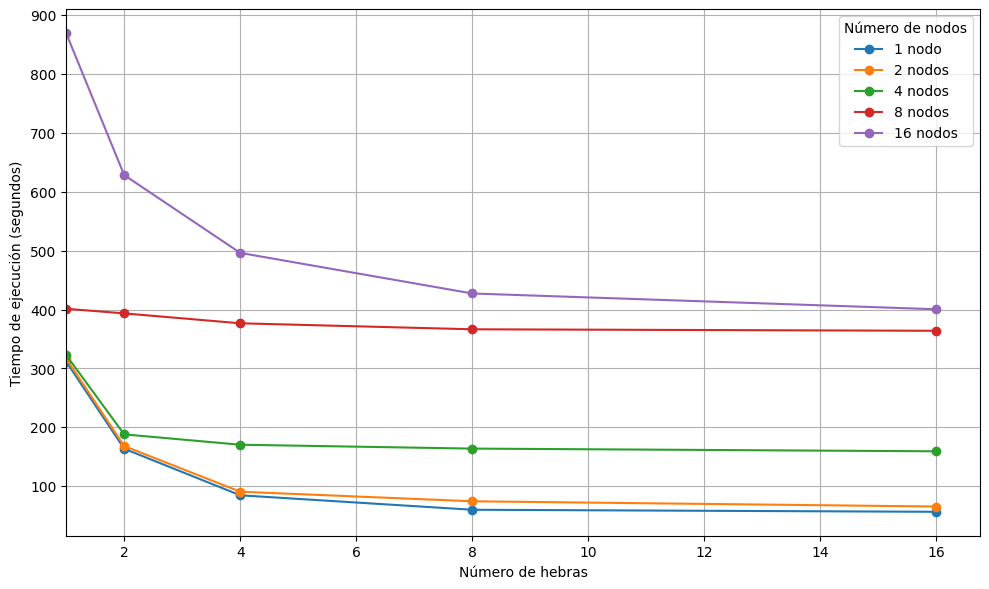
\includegraphics[width=0.8\textwidth]{imagenes/cap5/exploratory_gpu_limit_time.png}
    \caption{Gráfica de tiempo de ejecución en función del número de hebras por nodo, con la GPU limitada a un único nodo.}
    \label{fig:exploratory_gpu_limit_time}
\end{figure}

La figura \ref{fig:exploratory_gpu_no-limit_time} presenta los resultados de las ejecuciones exploratorias permitiendo el uso de la GPU en todos los nodos, evaluando así el comportamiento del sistema bajo esta configuración.

\begin{figure}[ht]
    \centering
    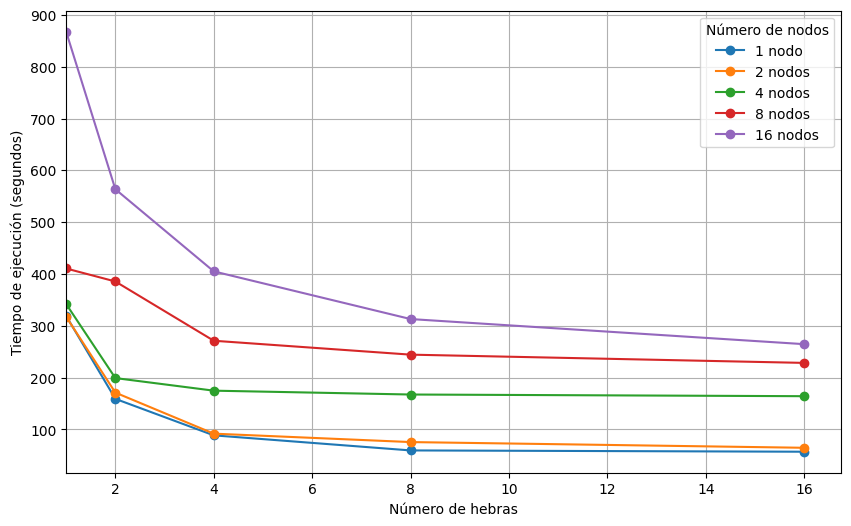
\includegraphics[width=0.8\textwidth]{imagenes/cap5/exploratory_gpu_no-limit_time.png}
    \caption{Gráfica de tiempo de ejecución en función del número de hebras por nodo, permitiendo el uso de la GPU en todos los nodos.}
    \label{fig:exploratory_gpu_no-limit_time}
\end{figure}

Las conclusiones que se pueden extraer de estas gráficas se pueden ver de manera más clara en la tabla \ref{tab:summary_nodes_threads_gpu}, donde se resumen los tiempos de ejecución para todas las combinaciones de nodos y hebras analizadas, tanto con la GPU limitada a un nodo como permitiendo su uso en todos los nodos.

\begin{table}[ht]
    \centering
    \scriptsize
    \setlength{\tabcolsep}{2pt}
    \renewcommand{\arraystretch}{1.1}
    \begin{tabular}{|c|c|c|c|c|}
        \hline
        \textbf{Nodos} & \textbf{Hebras} & \textbf{GPU 1 nodo (s)} & \textbf{GPU todos (s)} & \textbf{Var. (\%)} \\
        \hline
        1              & 1               & 311.68                  & 319.01                 & 2.35               \\
        1              & 2               & 163.59                  & 158.94                 & -2.84              \\
        1              & 4               & 84.49                   & 88.52                  & 4.77               \\
        1              & 8               & 59.91                   & 59.41                  & -0.83              \\
        1              & 16              & 56.45                   & 56.91                  & 0.81               \\
        2              & 1               & 316.92                  & 317.35                 & 0.14               \\
        2              & 2               & 168.14                  & 170.99                 & 1.70               \\
        2              & 4               & 90.58                   & 91.78                  & 1.32               \\
        2              & 8               & 74.30                   & 75.53                  & 1.66               \\
        2              & 16              & 65.40                   & 64.51                  & -1.36              \\
        4              & 1               & 322.77                  & 341.95                 & 5.94               \\
        4              & 2               & 187.98                  & 199.04                 & 5.88               \\
        4              & 4               & 170.38                  & 174.74                 & 2.56               \\
        4              & 8               & 163.80                  & 167.31                 & 2.14               \\
        4              & 16              & 159.22                  & 164.07                 & 3.05               \\
        8              & 1               & 401.33                  & 410.54                 & 2.29               \\
        8              & 2               & 393.50                  & 385.47                 & -2.04              \\
        8              & 4               & 376.68                  & 271.10                 & -28.03             \\
        8              & 8               & 366.47                  & 244.26                 & -33.35             \\
        8              & 16              & 363.94                  & 228.34                 & -37.26             \\
        16             & 1               & 869.40                  & 867.50                 & -0.22              \\
        16             & 2               & 628.49                  & 563.51                 & -10.34             \\
        16             & 4               & 496.28                  & 404.98                 & -18.40             \\
        16             & 8               & 427.30                  & 312.94                 & -26.76             \\
        16             & 16              & 400.48                  & 264.49                 & -33.96             \\
        \hline
    \end{tabular}
    \caption{Resumen de tiempos de ejecución para distintas combinaciones de nodos y hebras, comparando el uso de la GPU limitada a un nodo frente a su uso en todos los nodos.}
    \label{tab:summary_nodes_threads_gpu}
\end{table}

Para configuraciones con pocos nodos (1, 2 o 4), la diferencia entre utilizar la GPU en un único nodo o en todos los nodos resulta pequeña y variable. Las variaciones porcentuales oscilan entre valores positivos y negativos, pero en general se mantienen por debajo del 6\%. Esto indica que, en estos escenarios, no existe una ventaja clara ni consistente de emplear la GPU de forma compartida en todos los nodos.

A partir de 8 nodos, la ejecución con la GPU disponible en todos los nodos comienza a mostrar mejoras significativas, especialmente al incrementar el número de hebras. Por ejemplo, con 8 nodos y 16 hebras se observa una reducción del tiempo de ejecución del 37.26\%, mientras que con 16 nodos y 16 hebras la mejora alcanza el 33.96\%. Estas diferencias son consistentes y tienden a aumentar conforme crece el número de nodos y hebras.

En configuraciones con un número elevado de nodos y hebras, la opción de permitir el acceso a la GPU en todos los nodos se presenta como claramente superior, ya que maximiza el aprovechamiento de la capacidad de cómputo distribuido y reduce de manera significativa los tiempos de ejecución.

En resumen, para experimentos pequeños o con pocos nodos ambas opciones resultan comparables. Sin embargo, en experimentos de mayor escala y con configuraciones que involucran un alto número de nodos y hebras, la estrategia más eficiente y recomendable es habilitar el uso de la GPU en todos los nodos.

\subsection{Análisis de los experimentos preliminares}

A partir de los resultados obtenidos, se recomienda fijar el número de subpoblaciones en 8, ya que este valor representa un equilibrio óptimo entre eficiencia, utilización de recursos y escalabilidad en el entorno analizado.

En cuanto al número de hebras, los datos muestran que imponer un límite estricto puede restringir el aprovechamiento total de los recursos, especialmente en configuraciones multinodo. Por ello, se recomienda no limitar el número de hebras, permitiendo que el sistema utilice tantas como sean necesarias para maximizar el rendimiento.

Respecto al uso de la GPU, los experimentos indican que en configuraciones pequeñas las diferencias entre habilitarla en todos los nodos o solo en uno son mínimas. Sin embargo, en escenarios de mayor escala, habilitar su uso en todos los nodos aporta mejoras sustanciales en el tiempo de ejecución y en la eficiencia global. Por tanto, se establece como criterio general que la GPU esté disponible en todos los nodos.

En conjunto, estas decisiones proporcionan una base sólida y coherente para el diseño de los experimentos posteriores, asegurando que se exploten al máximo los recursos disponibles sin comprometer la comparabilidad de los resultados.

\section{Pruebas mononodo}

\subsection{Ejecución en Ubuntu en nativo}

\subsubsection{CPU}

En la figura \ref{fig:single-node_ubuntu_cpu_native_time} se muestra el tiempo de ejecución para la configuración de CPU en un único nodo con Ubuntu nativo.

\begin{figure}[H]
    \centering
    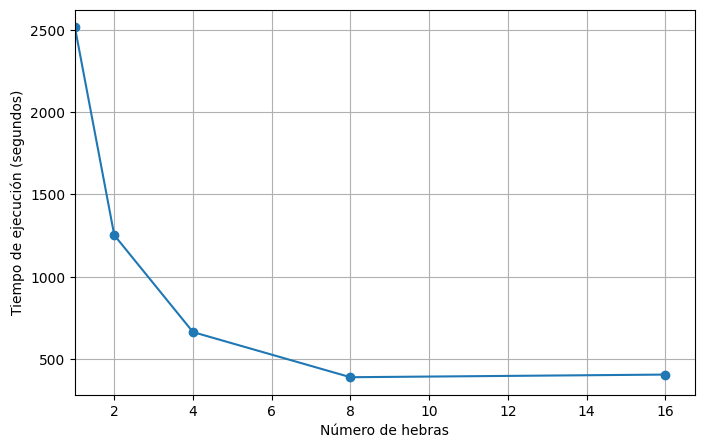
\includegraphics[width=0.8\textwidth]{imagenes/cap5/single-node_ubuntu_cpu_native_time.png}
    \caption{Tiempo de ejecución en función del número de hebras en Ubuntu nativo (CPU).}
    \label{fig:single-node_ubuntu_cpu_native_time}
\end{figure}

En la tabla \ref{tab:single-node_ubuntu_cpu_native} se presentan los tiempos de ejecución y la reducción porcentual respecto a una hebra.

\begin{table}[ht]
    \centering
    \begin{tabular}{|c|c|c|}
        \hline
        \textbf{Hebras} & \textbf{Tiempo (s)} & \textbf{$\Delta$\% vs 1 hebra} \\
        \hline
        1               & 2515.21             & 0.00                           \\
        2               & 1253.18             & -50.18                         \\
        4               & 664.69              & -73.57                         \\
        8               & 390.72              & -84.47                         \\
        16              & 406.76              & -83.83                         \\
        \hline
    \end{tabular}
    \caption{Tiempos de ejecución y reducción porcentual respecto a una hebra en Ubuntu nativo (CPU).}
    \label{tab:single-node_ubuntu_cpu_native}
\end{table}

El tiempo de ejecución disminuye drásticamente al aumentar el número de hebras, especialmente en el rango de $1$ a $8$ hebras. Con $2$ hebras, el tiempo se reduce prácticamente a la mitad ($-50.18\%$), y con $4$ hebras, a casi una cuarta parte del tiempo original ($-73.57\%$). El mayor beneficio se observa al pasar de $4$ a $8$ hebras, alcanzando una reducción del $-84.47\%$ respecto a una hebra. Sin embargo, al incrementar a $16$ hebras, el tiempo de ejecución es ligeramente superior al obtenido con $8$ hebras, lo que sugiere la aparición de saturación o sobrecarga en el sistema. Por tanto, el óptimo se alcanza con $8$ hebras, coincidiendo con el número de núcleos físicos disponibles en el sistema.

Estos resultados evidencian un buen escalado del rendimiento al aumentar el número de hebras en un entorno mononodo de ejecución nativa en Ubuntu utilizando únicamente la CPU.

\paragraph{CPU + GPU}

\subsection{Ejecución en contenedores de Ubuntu}
\paragraph{CPU}

\paragraph{CPU + GPU}

\subsection{Contenedores en contenedores de Windows}
\paragraph{CPU}

\paragraph{CPU + GPU}

\subsection{Contenedores en contenedores de Mac}
\paragraph{CPU}

\section{Pruebas multinodo}
\subsection{Ejecución en Ubuntu en nativo}
\paragraph{CPU}

\paragraph{CPU + GPU}

\subsection{Ejecución en contenedores de Ubuntu}
\paragraph{CPU}

\paragraph{CPU + GPU}

\subsection{Contenedores en contenedores de Windows}
\paragraph{CPU}

\paragraph{CPU + GPU}

\subsection{Contenedores en contenedores de Mac}
\paragraph{CPU}

\section{Pruebas de barrido de hebras}
\subsection{Ejecución en Ubuntu en nativo}
\paragraph{CPU}

\paragraph{CPU + GPU}

\subsection{Ejecución en contenedores de Ubuntu}
\paragraph{CPU}

\paragraph{CPU + GPU}

\subsection{Contenedores en contenedores de Windows}
\paragraph{CPU}

\paragraph{CPU + GPU}

\subsection{Contenedores en contenedores de Mac}
\paragraph{CPU}

